\documentclass[a4paper,11pt]{article}
\usepackage[utf8]{inputenc}
\usepackage[frenchb]{babel}
\usepackage{amssymb}
\usepackage{amsmath}
\usepackage{amsthm}
\usepackage{mathrsfs}
\usepackage{array}
\usepackage{graphicx}
\usepackage[usenames,dvipsnames]{color}
\usepackage{listings}
\usepackage{arydshln}
%\usepackage{slashbox}
\usepackage{subfigure}
\usepackage{pdflscape}
%\usepackage{cancel}
%\usepackage[bookmarks = false]{hyperref}
\usepackage[left=2cm, right=2cm, top=2cm, bottom=2cm]{geometry}

\newcommand{\ttsee}[1]{Voir \texttt{#1}\paragraph{}}
\newcommand{\ttseek}[1]{Voir package \texttt{#1}\paragraph{}}


% Initialisation de listings
%\definecolor{mymauve}{rgb}{0.63,0.13,0.94}
%\definecolor{mygreen}{rgb}{0.13,0.55,0.13}
%\definecolor{mybeige}{rgb}{0.99,0.99,0.86}
%\definecolor{mygris}{rgb}{0.8,0.8,0.8}
\definecolor{light-gray}{gray}{0.50}
\lstset{
    columns=flexible,
	%numbers = left,				% placement de la numérotation des lignes
	numberstyle = \small,        	% taille du numéro de ligne
	stepnumber = 1,              	% ???
	numbersep = 10pt,            	% taille de l'espace de séparation entre numéro de ligne et code
	showspaces = false,          	% montrer les espaces
	showstringspaces=false,         % enlever les espaces str
	showtabs = false,            	% montrer les tabulations
	tab = rightarrowfill,        	% ???
	tabsize=3,						% tabulation size
	language = Java,             	% langage utilisé
	basicstyle = \footnotesize\tt,	% ???
	captionpos = b,					% ???
	linewidth=\linewidth,			% largeur de la fenetre de code
	breaklines = true,				% ???
	commentstyle = \color{light-gray}, % définition de la couleur des commentaires
	%stringstyle = \color{mymauve},  % définition de la couleur des chaines de caractères
	%identifierstyle = \ttfamily,    % ???
	keywordstyle = \color{blue},	% définition de la couleur des mots clés
	%frame=single,
	%backgroundcolor=\color{mybeige},
	extendedchars=true				% étend les caractères pouvant être utilisés
}

%\author{Mormont Romain}
%\title{Synthèse : Base de données (Pierre Wolper)}
%\date{Année académique 2013-2014}

\begin{document}
\rule{1\linewidth}{1px}
{ \sc
\begin{center}
{\small Université de Liège}\\
{\small Faculté des Sciences Appliquées}

\end{center}

\vfill
\begin{center}

{\Huge Introduction to computer networking {\LARGE \tt [INFO0010-1]}\\}
\end{center}
\begin{center}
{\Huge Projet 2 : Rapport}
\end{center}
\begin{center}
Mormont Romain, Servais Fabrice\\
{\small 3$^{\text{ème}}$  bachelier ingénieur civil, orientation ingénieur civil}\\
{\small Options \textit{informatique} et \textit{électricité et électronique}}\\
{\small s110940, s111093}
\end{center}

\vfill
\begin{center}
Année académique 2013-2014\\
\end{center}
}
\rule{1\linewidth}{1px}
\newpage
\tableofcontents
\newpage
\section{Software architecture}
Le problème a été divisé en différents sous-problèmes que nous allons expliciter dans leur ordre temporel.

	\subsection{Vue globale de la solution}

	\subsubsection{Initialisation du \textit{Gateway}}
Une instance de \texttt{Server} est créée au lancement de cette classe. Celle-ci crée une instance de \texttt{HTTPServer} et \texttt{ConfigurationServer} afin d'accepter les connexions entrantes vers le \textit{Gateway} et la plate-forme de configuration. Elle récupère aussi le singleton \texttt{Displayer} servant à afficher des messages dans la console. Nous ne détaillerons pas la plate-forme de configuration.

	\subsubsection{Récupération des connexions entrantes}
La classe \texttt{HTTPServer} récupère les connexions entrantes et lance un thread (si possible par la thread-pool) pour chacune d'entre-elles par l'intermédiaire de la classe \texttt{HTTPClientRequestThread} et ce, après l'acceptation de connexion du socket.

	\subsubsection{Gestion des requêtes}
	La classe \texttt{HTTPClientRequestThread} instancie un objet \texttt{HTTPRequest} en prenant le socket en argument. Celui-ci va récupérer la requête du navigateur et la parser pour en récupérer les différentes informations, notamment la méthode et le chemin.

\paragraph{}

On récupère alors l'adresse IP du \textit{Gateway} qui va être utile lors du remplacement des liens, et l'on donne la requête récupérée à un nouvel objet de classe \texttt{GatewayRequestDecoder} qui va se charger de décoder la requête, c'est-à-dire récupérer l'adresse du site auquel l'utilisateur souhaite accéder et les éventuels paramètres (\texttt{forceRefresh}). On vérifie ensuite si l'adresse est correcte et que le format du fichier auquel on veut accéder est géré.

\paragraph{}

Pour le chemin donné, on regarde si la page est déjà contenue dans le cache et si celle-ci doit être rafraîchie dû au timeout ou à l'éventuel argument \texttt{forceRefresh}. Selon les cas, on va rechercher la page dans le cache ou sur le serveur distant. Dans ce cas-là, la méthode \texttt{getPageFromRemote(URL)} établit la connexion avec le serveur avec la classe \texttt{HttpURLConnection} et récupère le contenu de la page. Les liens de la page sont alors filtrés afin de les rediriger vers le \textit{Gateway}. Les balises \texttt{img}, \texttt{link}, \texttt{frame} et \texttt{script} sont aussi filtrées afin de bypasser le \textit{Gateway}. 

\paragraph{}

On clone ensuite la page récupérée (afin de ne pas altérer la page originale contenue dans le cache) puis on filtre la page en fonction des mots-clés interdits. Cette étape est réalisée après la récupération de la page du cache ou du serveur distant. En effet, il est possible que la page ait été modifiée sur le serveur distant pendant le temps où celle-ci se trouvait dans le cache, amenant possiblement des mots-clés interdits et devant provoquer une censure, ce qui n'aurait alors pas été le cas, jusqu'au timeout dans le cache. Si la page doit être censurée, on renvoie une page informant d'utilisateur qu'il ne peut pas accéder à la page. Sinon, on envoie une réponse HTTP contenant la page voulue ou pas selon si on répond à une requête GET ou HEAD.

\begin{landscape}
	\begin{figure}
		\center
		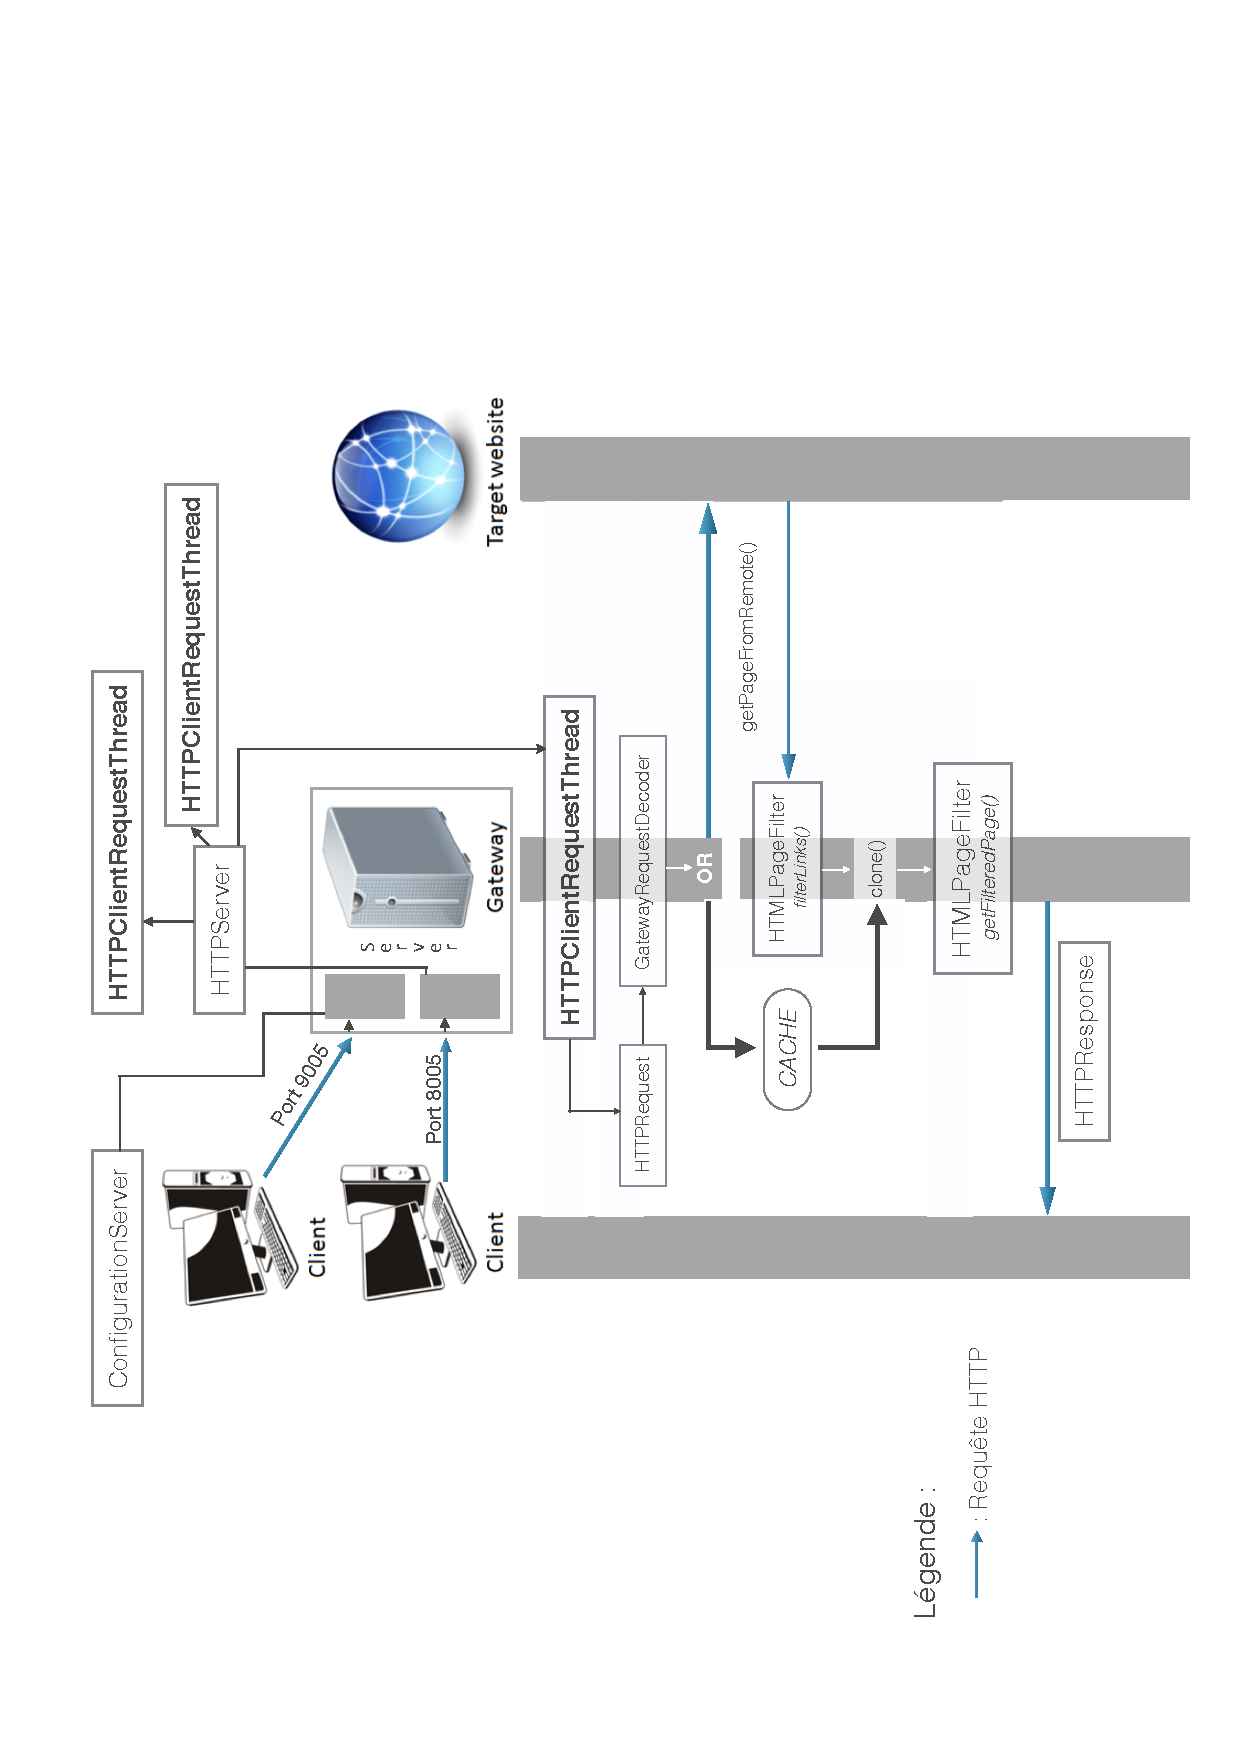
\includegraphics[scale=0.85]{schema-general}
		\caption{Schéma général de l'implémentation}
		\label{fig:schema_general}
	\end{figure}
\end{landscape}

	\subsection{Erreurs renvoyées par le \textit{Gateway}}
Voici une liste de différentes erreurs renvoyées par le \textit{Gateway} ainsi que l'action qui les a déclenchées : 
\begin{itemize}
	\setlength{\itemsep}{6pt}
	\item \textbf{Erreur 400 - Bad Request} : La requête du client n'a pu être lue (dû à la variable \texttt{s} manquante dans l'URL, argument de \texttt{s} vide,...)
	\item \textbf{Erreur 500 - Internal Server Error} : Lorsqu'une erreur lors du parsage du code HTML a été rencontrée.
	\item \textbf{Erreur 501 - Not Implemented} : La requête que l'on reçoit n'est ni GET ni HEAD ou lorsque le format de la page demandée n'est pas prise en charge.
	\item \textbf{Erreur 502 - Bad Gateway} : Le serveur distant n'a pas pu être atteint.
	\item \textbf{Erreur 504 - Gateway Timeout} : Le serveur distant a été trop lent à joindre ou à répondre.
\end{itemize}
\paragraph{}
Lorsque le serveur distant répond et qu'il renvoie un code d'erreur HTTP, le \textit{Gateway} transmet cette erreur au client.
\subsection{Interaction avec le HTML}
Nous avons voulu éviter, lors du traitement des liens et des mots clés, de devoir manipuler une longue chaîne de caractère contenant le code HTML. Ainsi faciliter ces manipulations, nous avons développé un package \texttt{html} contenant une série de classes utiles. 
\subsubsection{Éléments HTML}
\ttseek{html}
Tout d'abord, nous avons développé une classe \texttt{HTMLPage} qui contient notre représentation interne d'une page.
Ensuite, nous avons développé une classe abstraite \texttt{HTMLElement} pour représenter un élément HTML et des classes héritant de cette dernière pour représenter les éléments concrets. Notre classification ainsi que les classes associées à chaque élément sont données dans la Table \ref{tab:htmlelement}.
\begin{table}[h]
	\center
	\begin{tabular}{|c|p{0.33\linewidth}|c|}
		\hline
		\textbf{Élément} & \multicolumn{1}{c|}{\textbf{Forme}} & \textbf{Classe}\\
		\hline
		Balise ouvrante & \texttt{<tag\_name attr="value" ...>} & \texttt{HTMLOpeningTag}\\
		\hline
		Balise fermante & \texttt{</tag\_name>} & \texttt{HTMLClosingTag}\\
		\hline
		Balise commentaire & \texttt{<!-- ... -->} & \texttt{HTMLComment} \\
		\hline
		Contenu & Tout contenu ne se trouvant pas à l'intérieur d'une balise & \texttt{HTMLContent}\\
		\hline
		Attribut d'une balise ouvrante & \texttt{attr="value"} & \texttt{HTMLAttribute}\\
		\hline
	\end{tabular}
	\caption{Classification des \texttt{HTMLElement}}
	\label{tab:htmlelement}
\end{table}
\paragraph{} Ces classes définissent toutes les méthodes permettant de consulter ou de modifier leurs différentes caractéristiques. Par exemple, la classe \texttt{HTMLContent} définit une méthode permettant de remplacer chaque caractère d'un mot donné par un autre caractère. Ou encore, la classe \texttt{HTMLPage} définit une méthode permettant de récupérer toutes les balises ouvrantes ayant le même nom.
\paragraph{}
Notre représentation interne d'une page est une liste d'objets \texttt{HTMLElement}.
\subsubsection{Parser}
\ttseek{html.parser}
Afin de pouvoir exploiter les outils définis précédemment, il est nécessaire de convertir un code HTML en objets. Pour ce faire nous avons développé la classe \texttt{HTMLParser} permettant de pratiquer une analyse lexicale du code sur base d'une machine d'états finie.
\paragraph{}
La classe est composée, entre autres, de plusieurs méthodes chacune chargée de parser un élément HTML particulier (voir Table \ref{tab:htmlelement}) :
\begin{itemize}
	\item \texttt{parseOpeningTag} : balise ouvrante (machine d'états donnée dans la Figure \ref{ref:pars_opening})
	\item \texttt{parseClosingTag} : balise fermante
	\item \texttt{parseContent} : contenu (machine d'états donnée dans la Figure \ref{fig:pars_content})
	\item \texttt{parseAttribute} : attribut (et sa valeur s'il y en a une) (machine d'états donnée dans la Figure \ref{ref:pars_opening})
	\item \texttt{parseComment} : commentaire
\end{itemize}
\paragraph{}
Ces méthodes sont coordonnées par les méthodes \texttt{parseTag} et \texttt{parseHTML}. La première, en fonction de la balise rencontrée, passe la main à \texttt{parseOpeningTag}, \texttt{parseClosingTag} ou \texttt{parseComment} et la seconde, en fonction du caractère, passe la main à \texttt{parseTag} ou \texttt{parseContent}.
\paragraph{}
A la fin de l'analyse, le parser a construit une liste de \texttt{HTMLElement} qui constitue notre représentation interne du code dans \texttt{HTMLPage}.
\subsubsection{Filtre}
\ttseek{html.filter}
Le filtrage des liens nous a posé pas mal de problèmes. En effet, étant donné la permissivité du langage HTML, les liens peuvent être relatifs ou absolus, avec ou sans protocole,... De plus, il se peut que le contenu de la balise \texttt{href} ne soit pas un lien vers une page web mais un lien vers une adresse mail (\texttt{mailto:...}) ou vers une fonction javascript (\texttt{javascript:...}). Enfin, l'adresse de référence des liens relatifs peut être différente de la racine du serveur selon que la balise \texttt{<base ...>} ait été déclarée ou non à l'intérieur des balises \texttt{head}. 
\paragraph{}
Étant donnée la complexité du problème, il nous a semblé judicieux de créer une classe dédiée à sa résolution : la classe \texttt{LinkFilter}. En plus de reconstruire une url absolue sur base de l'adresse d'une page web et d'un lien, cette classe permet aussi d'encoder une url et de construire le lien complet dirigeant vers le \textit{Gateway}. Cette classe est utilisée dans la classe \texttt{HTMLPageFilter}.
\paragraph{}
Cette dernière classe permet aussi de filtrer la page selon les critères précisés dans l'énoncé. Les différents états sont repris dans l'énumération \texttt{PageGatewayStatus}.

\section{Multi-thread coordination}
L'accès au cache est \textit{thread-safe}. En effet, le cache est implémenté avec la classe \texttt{ConcurrentHashMap} qui est \textit{thread-safe}. De plus, nous avons ajouté l'attribut \texttt{synchronized} aux méthodes de \texttt{Cache} agissant avec le cache. Si deux threads tentent d'accéder à une même page se trouvant dans le cache, ces deux threads recevront la même page, sans incohérence.
\paragraph{}
Le seul moment où le cache est modifié est lors l'insertion ou la mise à jour d'une page lorsqu'un utilisateur demande cette page. Supposons que deux utilisateurs souhaitent accéder à la même page ne se trouvant pas dans le cache. Les deux threads demanderont tous les deux au serveur distant après la page, filtreront les liens et attributs cités au point 1.1.3, et tenteront de l'insérer dans le cache. Un premier y parviendra avant l'autre, et ce deuxième ajout aura pour effet d'écraser la précédente. Cependant, ceci n'est pas un problème puisque l'on peut supposer que la page n'a pas changé entre les moments où les utilisateurs ont demandé la page, celle-ci est alors dans le même état pour chacun des threads.
\paragraph{}
On peut noter aussi que le clonage de l'élément contenu dans le cache ajoute un niveau de sécurité supplémentaire car, lorsque l'on modifie la page, le cache n'est pas modifié, cela n'a donc pas d'incidence sur les autres threads.

\section{Limits and possible improvements}

	\subsection{Sécurité}
Les scripts Javascript sont ignorés, or ceux-ci pourraient amener des mots-clés interdits ou des liens qui ne seront donc pas redirigés vers le \textit{Gateway}. Un parsage de ces scripts résoudrait le problème. 

	\subsection{Utilisation}
Certains types de fichiers ne sont pas accessibles depuis le \textit{Gateway} (e.g. pdf, zip,...) et les images bypassent celui-ci. On pourrait améliorer le \textit{Gateway} en implémentation une gestion de ces fichiers.
\paragraph{}
Les requêtes autres que GET ou HEAD ne sont pas gérées. Une amélioration possible serait de toutes les implémenter.

\section{Reference websites}

	\subsection{Succès}

	\subsection{Échecs}






\newpage
\appendix
\section{Machine d'états}
\subsection{Parsing des balises ouvrantes}
La représentation graphique est donnée à la Figure \ref{ref:pars_opening}.

\begin{figure}[h]
	\center
	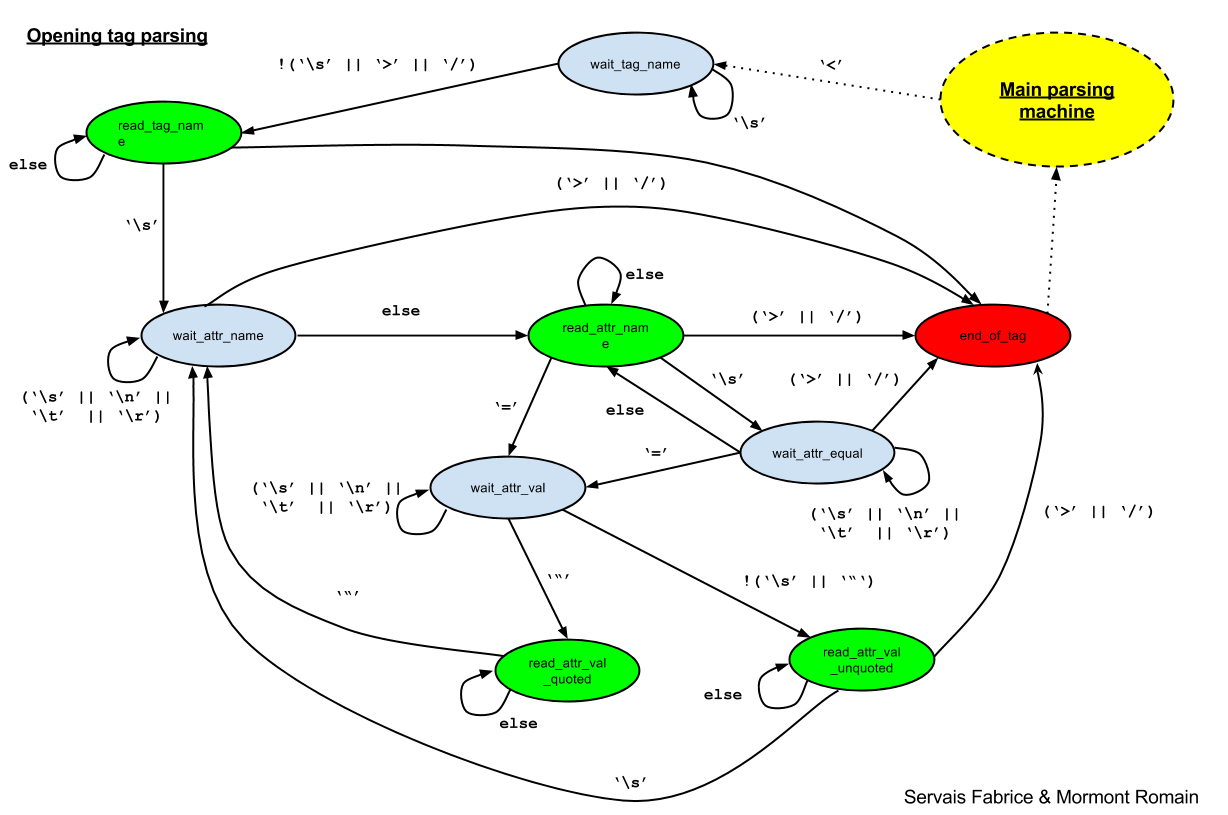
\includegraphics[scale=0.35]{parseOpeningTagFSM.png}
	\caption{Parsing des balises ouvrantes}
	\label{ref:pars_opening}
\end{figure}

\paragraph{}
Les différents états :
\begin{itemize}
	\item \texttt{wait\_tag\_name} : en attente du début du nom de la balise 
	\item \texttt{read\_tag\_name} : lecture du nom de la balise
	\item \texttt{wait\_attr\_name} : en attente d'un nom d'attribut
	\item \texttt{read\_attr\_name} : lecture du nom d'un attribut
	\item \texttt{wait\_attr\_equal} : en attente du \texttt{=} suivant l'attribut
	\item \texttt{wait\_attr\_val} : en attente de la valeur de l'attribut
	\item \texttt{read\_attr\_val\_unquoted} : lecture d'un attribut sans apostrophe ou guillemet
	\item \texttt{read\_attr\_val\_quoted} :  lecture d'un attribut avec apostrophe ou guillemet
\end{itemize}
\paragraph{}
Ce modèle d'état ne prend pas en compte les cas où le nom d'attribut est entouré de guillemets (peut arriver pour certaines balises \texttt{!DOCTYPE}). Ce cas a néanmoins été pris en compte dans le code.

\subsection{Parsing du contenu}
La représentation est donnée à la Figure \ref{fig:pars_content}.
\begin{figure}
	\center
	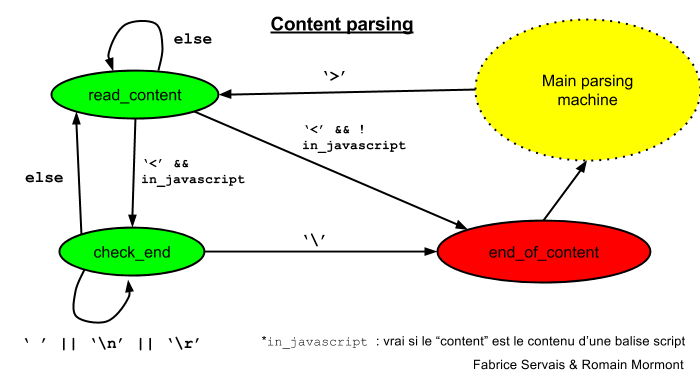
\includegraphics[scale=0.5]{parseContentFSM.png}
	\caption{Parsing d'un contenu}
	\label{fig:pars_content}
\end{figure}
\paragraph{}
Les différents états :
\begin{itemize}
	\item \texttt{read\_content} : lecture du contenu
	\item \texttt{check\_end} : dans le cas où le contenu est un code javascript (placé dans des balises \texttt{script}), il se peut que le chevron fermant ne soit pas le début de la balise fermante \texttt{</script>}. Il faut s'assurer que c'est bien le cas avant d'achever le parsing du contenu.
\end{itemize}

\end{document}
